\documentclass[a4paper, 11pt]{article}

\usepackage[utf8]{inputenc}
\usepackage{amsmath,amsthm,amssymb}
\usepackage{mathtools}
\usepackage{geometry} 
\usepackage{marvosym}
\usepackage[toc,titletoc,title]{appendix}
\usepackage[hidelinks]{hyperref}
\usepackage{framed}
\usepackage{enumitem}
\usepackage{parskip}

\usepackage{xcolor}
\hypersetup{
	colorlinks,
	linkcolor={red!50!black},
	citecolor={red!50!black},
	urlcolor={red!50!black}
}

\makeatletter
\def\thm@space@setup{%
	\thm@preskip=5mm
	\thm@postskip=\thm@preskip % or whatever, if you don't want them to be equal
}
\makeatother

% bold title for optional title in theorems
\makeatletter
\def\th@plain{%
	\thm@notefont{}% same as heading font
	\itshape % body font
}
\def\th@definition{%
	\thm@notefont{}% same as heading font
	\normalfont % body font
}
\makeatother

\theoremstyle{plain}
\newtheorem{theorem}{Theorem}
\newtheorem{lemma}[theorem]{Lemma}
\newtheorem{collorary}[theorem]{Collorary}
\newtheorem{proposition}{Proposition}


\theoremstyle{definition}
\newtheorem{definition}[theorem]{Definition}
\newtheorem*{example}{Example}
\newtheorem*{remark}{Remark}

% roman number
\newcommand{\rom}[1]{\uppercase\expandafter{\romannumeral #1\relax}}



\begin{document}

\title{Proofs from the Lebesgue theory}
\author{Viet Duc Nguyen\\ Technical University of Berlin\\ Analysis III}
\maketitle
\tableofcontents

\setcounter{section}{7}
\section{Properties of measurable functions}
\begin{itemize}
	\item Let $f,g: \Omega \to \mathbb R$ be $\mathcal F$-measurable. Then $f+g$, $f^2$ and $fg$ are measurable.
	\begin{proof}[Proof]
		We want to show that $f+g$ is measurable. It is measurable if 
		$$\forall a \in \mathbb R: \{ f+g < a \} \in \mathcal F.$$ 
		
		\textit{Idea:} First, we will show that $\{ h < i \} \in \mathcal F$ for measurable functions $h$ and $i$. Setting $h \coloneqq f$ and $i \coloneqq a-g$ gives the result because $f$ is measurable and $a-g$ is measurable.
		
		Note: We cannot directly set $h \coloneqq f+g$ and $i \coloneqq a$, for we do not know if $f+g$ is measurable!
		
		Now, let's show that $\{ h < i \}$ is measurable if $h,i \in \mathcal F$. It holds
		\[
			\{ h < i \} = \bigcup_{q \in \mathbb Q} \{ h < q \} \cap \{ q < i \} \in \mathcal F,
		\]
		for $\{ h < q \} \in \mathcal F$ and $\{ q < i \} \in \mathcal F$ (after the assumption).
		
		Geometrically speaken, we have divided the half plane below the line $f+g = a$ in countably many boxes.
		\begin{figure}
		\begin{center}
			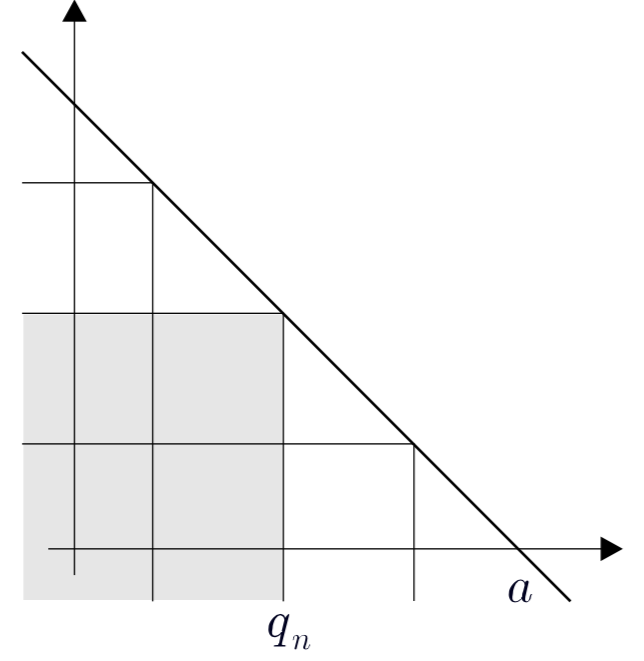
\includegraphics[scale=0.25]{boxes.png}
			\caption{The subplane below the line is covered by boxes. Source: Lecture notes 2018, Prof. Charles Batty}
		\end{center} 
		\end{figure}
		
		\textit{Bonus:} we show $\{ h \leq i \}$ is measurable by using that $\{ h < i\}$ is measurable. It holds
		\[
			\{ h \leq i \} = \bigcap_{\substack{q \in \mathbb Q\\q > 0}} \{ h < i +q \} \in \mathcal F.
		\]
		
		We show that $f^2$ is measurable, and if that holds true, we can easily show that $fg$ is measurable because $fg = \frac{1}{4}\Big((f+g)^2-(f-g)^2\Big)$. Note that $f-g$ is measurable because $-g$ is measurable and thus $f+(-g)$.
		
		Consider $\{ f^2 > a \}$. If $a < 0$, then this set is $\Omega$, which is indeed measurable. For $a > 0$:
		\[
			\{ f^2 > a \} = \{ f > \sqrt a \} \cup \{ f < -\sqrt a \} \in \mathcal F,
		\]
		for $ \{ f > \sqrt a \}$ and $ \{ f < -\sqrt a \}$ are measurable.
	\end{proof}

	\item Let $\{f_n\}_{n \in \mathbb N}$ be a sequence of measurable functions in $\mathbb R$. Then, $\sup f_n$, $\inf f_n$, $\lim \sup f_n$ and $\lim \inf f_n$ are measurable.
	\begin{proof}
		We show that $\sup f_n$ is measurable. For any $k \in \mathbb N_{\geq 1}$ and $a \in \mathbb R$, it holds:
		\[
			\{ x : (\sup_{n \geq k}f_n)(x) > a \} = \bigcup_{n \geq k} \{ x : f_n(x) > a \} \in \mathcal F.
		\]
		Similarly,
		\[
			\{ x: (\inf_{n \geq k}f_n)(x) \geq a \} = \bigcap_{n \geq k}\{ x: f_n(x) \geq a \} \in \mathcal F.
		\]
		Note that we must take $\geq$ since the intersection of open sets may not be open. Another idea to show that $\inf$ is measurable: $\inf(f_n) = -\sup(-f_n)$. 
		
		Now,
		\[
			\lim \sup f_n = \inf\limits_{k \in \mathbb N} \sup\limits_{n \geq k}f_n \in \mathcal F \quad \text{and} \quad \lim \inf f_n = \sup_{k \in \mathbb N} \inf_{n \geq k} f_n \in \mathcal F,
		\]
		because as shown $\inf f_n$ and $\sup f_n$  is measurable for any sequence $(f_n)_{n \in \mathbb N}$ of measurable functions.
		
		Alternatively, $\{ x : (\sup_{n \geq k}f_n)(x) \leq a \} = \bigcup_{n \geq k} \{ x : f_n(x) \leq a \} \in \mathcal F$ (note that we must use $\leq$).
		
		Note that, we shall check that $\{ x : (\sup f)(x) = \infty \} \in \mathcal F$, since $\sup f$ is a numerical function. The case is omitted, however it is easy to show. 
	\end{proof}

	\item $f^+,f^-$ and $|f|$ are measurable if $f$ is measurable.
	\begin{proof}
		The positive part is defined as $f^+(x) \coloneqq \begin{cases}
		f(x),  &f(x) \geq 0\\
		0, & f(x) < 0
		\end{cases} = \max\{f(x),0\}$.
		Consider the characteristic function $\chi_A$ where $A = \{ f \geq 0 \}$. Since $A$ is a measurable set, $\chi_A$ is a measurable function. Thus, the product $f \cdot \chi_A$ is measurable, since $f$ is measurable, and so is $f^+(x) = f\chi_A \in \mathcal F$.
		
		Similarly, $f^- = (-f)^+$ is measurable, since $-f$ is measurable.
		
		The absolute value of $f$ can be stated as $|f| = f^+ + f^-$, which is measurable as a sum of two measurable functions.
	\end{proof}

	\item $\max(f,g), \min(f,g)$ are measurable if $f$ and $g$ are measurable.
	\begin{proof}
		$\{ x : \max\{f(x),g(x)\} > a \} = \{ x : f(x) > a \} \cup \{ x : g(x) > a \} \in \mathcal F$. Now, it holds that $\min\{f,g\} = -\max\{-f,-g\} \in \mathcal F$.
	\end{proof}

\end{itemize}

\end{document}
